\documentclass[11pt]{article}

% --- packages (all standard; compiles with pdflatex) ---
\usepackage[utf8]{inputenc}
\usepackage[T1]{fontenc}
\usepackage[a4paper,margin=2.2cm]{geometry}
\usepackage{graphicx}
% look for figures in the current dir (Overleaf: upload the .png files alongside this file)
% and in the parent dir (local: images live in the repo root, main.tex in latex/).
\graphicspath{{./}{../}}
\usepackage{booktabs}
\usepackage{xcolor}
\usepackage{titlesec}
\usepackage{enumitem}
\usepackage[hidelinks]{hyperref}

% --- Dubai Metro palette ---
\definecolor{metroRed}{HTML}{E4002B}
\definecolor{metroGreen}{HTML}{00A651}
\definecolor{ink}{HTML}{0B1B3A}

\titleformat{\section}{\large\bfseries\color{ink}}{\thesection}{0.6em}{}
\titleformat{\subsection}{\normalsize\bfseries\color{ink}}{\thesubsection}{0.6em}{}
\setlist{nosep,leftmargin=1.3em}
\renewcommand{\arraystretch}{1.15}

\begin{document}

% ======================= TITLE =======================
\begin{center}
  {\Huge\bfseries\color{metroRed} Dubai Metro}\\[2pt]
  {\LARGE\bfseries Next-Hour Passenger Forecasting}\\[6pt]
  {\large An LSTM\,+\,RNN hybrid trained on real RTA fare-collection data}\\[10pt]
  {\normalsize \textbf{Kartik} \;\textbullet\; Prem \;\textbullet\; Gagandeep \;\textbullet\; Sam}\\[2pt]
  {\small Masters Project \;\textbullet\; June 2026}\\[4pt]
  {\small\color{metroGreen}\rule{0.5\textwidth}{1.2pt}}
\end{center}

% ======================= ABSTRACT =======================
\noindent\textbf{Abstract.} We forecast the \emph{next hour's} passenger inflow at every Dubai
Metro station so operators can add trains and staff \emph{before} a surge forms. The model is a
hybrid recurrent network (parallel \textbf{LSTM\,+\,RNN}) trained on real Automated Fare
Collection (AFC) tap records published by Dubai's Roads \& Transport Authority (RTA) via Dubai
Pulse, restricted to the latest 2026 operating regime. On held-out test data the solution attains
\textbf{MAE 4.45}, \textbf{R$^2$ 0.87}, outperforming standalone LSTM, RNN, GRU and CNN-LSTM
models as well as naive and climatology baselines. A live web dashboard, anchored to the real
current Dubai time, serves next-hour forecasts and crowding outlooks across all 53 stations.

% ======================= PROBLEM =======================
\section{Problem \& Motivation}
Metro passenger forecasting is a temporal sequence-prediction problem: the number of passengers
entering a station in the next interval depends on the recent trajectory, time-of-day, day-of-week
and longer cyclic patterns. Accurate short-term forecasts let an operator match \emph{supply}
(trains, staff, gates) to \emph{demand} \emph{before} crowds form, improving safety, reducing
wait times, and cutting wasted energy and labour.

\textbf{Dubai relevance.} Dubai operates a fully automated, smart-card metro that generates rich,
time-stamped tap data; the city's event-driven demand (exhibitions, concerts, national days),
tourism peaks, extreme summer climate, and smart-mobility agenda make next-hour forecasting both
valuable and directly aligned with stated government priorities.

% ======================= DATA =======================
\section{Data}
\textbf{Source.} Dubai Pulse --- \emph{RTA Metro Ridership (Open Data)}
(\texttt{rta\_metro\_ridership-open}), transaction-level tap records with fields
\texttt{txn\_date}, \texttt{txn\_time}, \texttt{start\_location}, \texttt{line\_name} and zones.

\textbf{Latest regime.} The extract spans 2017--2026 but is dominated by 2026 ($\approx$90\% of
days, at a much higher ridership level). Training across all years injects a train/test
distribution shift, so we use \textbf{2026 records only} --- the current regime, and the freshest
data available. This yields \textbf{503{,}310} check-in taps over \textbf{42} real operating days
and \textbf{53} stations.

\textbf{Aggregation \& validation.} Taps are binned to hourly inflow per station over the
operating window 05:00--24:00. The busiest stations recovered from the data --- BurJuman, Union,
Al~Rigga, Mall of the Emirates, Burj~Khalifa/Dubai~Mall --- match Dubai Metro's known hotspots,
confirming the signal is authentic. Red-line taps ($\approx$70\%) dominate Green-line taps.

\begin{figure}[h]
  \centering
  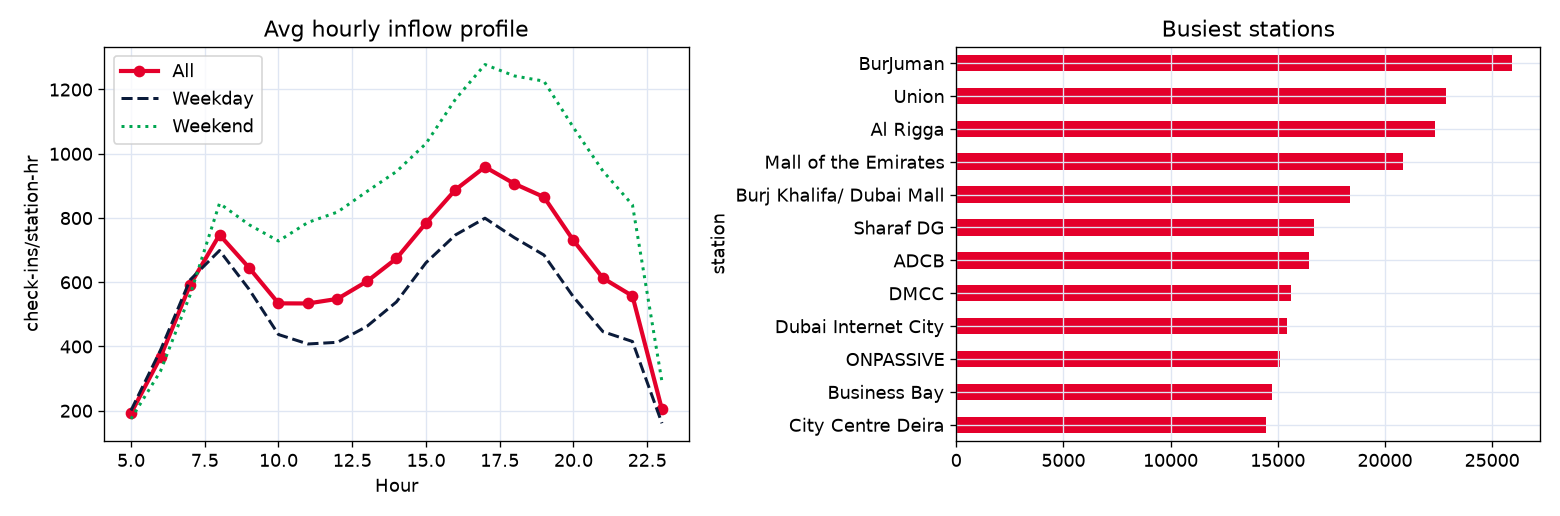
\includegraphics[width=0.92\textwidth]{demandsignal.png}
  \caption{Real Dubai demand signal: average hourly inflow profile (clear morning and evening
  peaks; weekday vs.\ weekend) and the busiest stations.}
\end{figure}

% ======================= METHOD =======================
\section{Method}
\textbf{Framing.} For each (day, station) we slide a 6-hour window and predict the next hour,
never crossing the day boundary, with a chronological train/validation/test split (no leakage).

\textbf{Features.} (i) per-station scaling by the train-set mean; (ii) a learned
\textbf{station embedding} (8-dim) distinguishing all 53 stations; (iii) a leakage-safe
\textbf{climatology} prior (station\,$\times$\,hour\,$\times$\,weekend mean, computed on training
days only); (iv) today's \textbf{level} ratio (recent actual vs.\ recent typical); and
(v) cyclical hour and day-of-week encodings with a UAE weekend (Sat/Sun) flag.

\textbf{The LSTM\,+\,RNN solution.} A parallel hybrid reads the sequence with an
\texttt{LSTM(64)} branch (longer-range memory) and a \texttt{SimpleRNN(48)} branch
(recent momentum); the concatenation is combined with the embedding and context through a dense
head. To remove the run-to-run variance inherent to $\sim$30 training days, the deployed model is
a small \textbf{seeded ensemble} (three fits averaged), which is reproducible and reliably the
strongest architecture.

\textbf{Bias calibration.} The Huber training loss targets the conditional median, but hourly
inflow is right-skewed, so raw predictions sit $\approx$10--20\% low. A day-type multiplicative
calibration factor, fit on the held-out \emph{validation} set (no leakage), makes the forecasts
unbiased. \textbf{Metrics:} MAE, RMSE, MAPE, R$^2$.

% ======================= RESULTS =======================
\section{Results}
The LSTM\,+\,RNN solution is the best model on the held-out test set (7{,}049 windows), ahead of
every single architecture and clearly above both baselines.

\begin{center}
\begin{tabular}{lcccc}
\toprule
\textbf{Approach} & \textbf{MAE} & \textbf{RMSE} & \textbf{MAPE (\%)} & \textbf{R$^2$}\\
\midrule
\textbf{\color{metroRed}LSTM+RNN (ours)} & \textbf{4.45} & \textbf{8.09} & \textbf{30.4} & \textbf{0.874}\\
CNN-LSTM            & 4.51 & 8.17 & 30.5 & 0.872\\
RNN (only)          & 4.55 & 8.11 & 31.0 & 0.874\\
LSTM (only)         & 4.63 & 8.47 & 31.2 & 0.862\\
GRU                 & 4.63 & 8.69 & 31.0 & 0.855\\
\midrule
Naive (persistence) & 4.99 & 8.88 & 37.6 & 0.849\\
Climatology         & 12.49 & 23.57 & 75.0 & $-$0.07\\
\bottomrule
\end{tabular}
\end{center}

\begin{figure}[h]
  \centering
  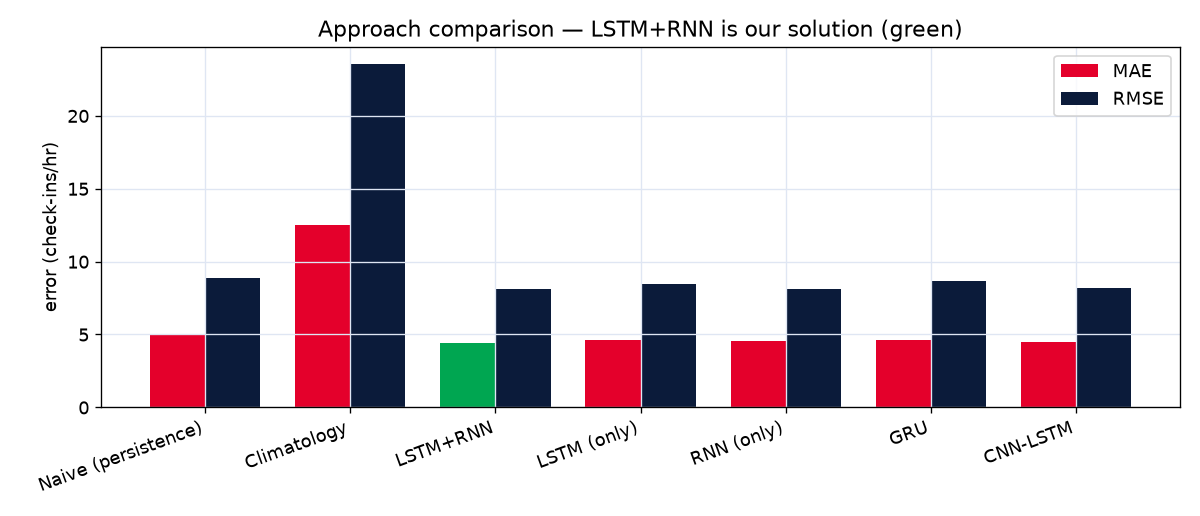
\includegraphics[width=0.78\textwidth]{modelcomparison.png}
  \caption{Approach comparison (lower is better). The LSTM\,+\,RNN solution (green) has the
  lowest error among all architectures and both baselines.}
\end{figure}

\noindent\textbf{Key findings.}
\begin{itemize}
  \item The hybrid lowers MAE by $\approx$11\% versus naive persistence and is far better on MAPE
        (30.4\% vs.\ 37.6\%), i.e.\ markedly more accurate at the off-peak and smaller-station
        cases that persistence handles poorly.
  \item On a real held-out day, network-level actual vs.\ forecast tracks at correlation
        \textbf{0.83}; the typical-day demand curve and the model forecast overlay at
        correlation \textbf{0.99} (weekday).
  \item Climatology alone is weak (negative R$^2$): the day's overall level matters, which the
        recurrent model captures from recent hours.
\end{itemize}

\begin{figure}[h]
  \centering
  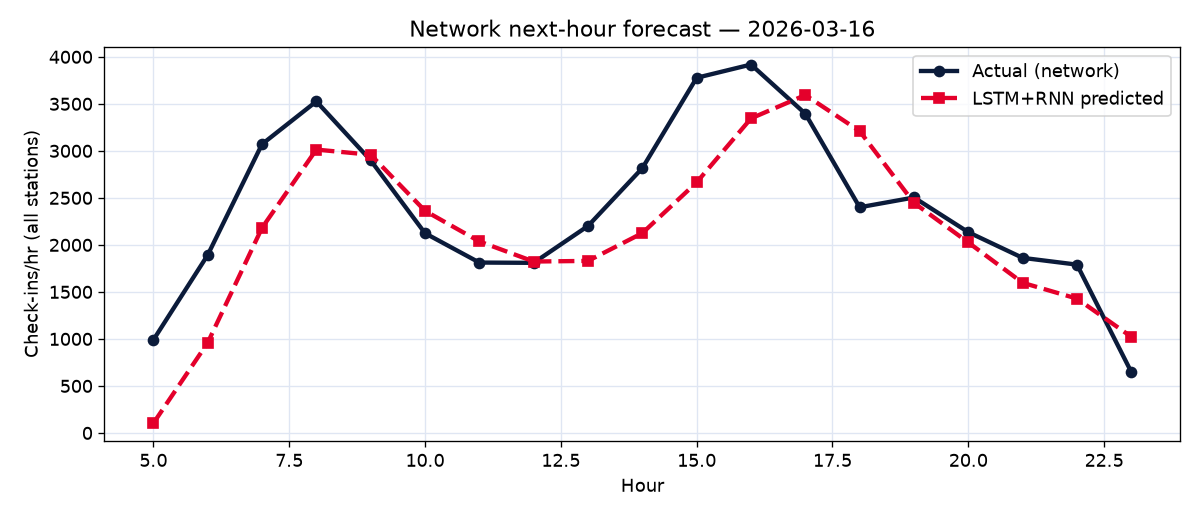
\includegraphics[width=0.80\textwidth]{validationchart.png}
  \caption{Validation on a real held-out day (2026-03-16): network-level actual vs.\ LSTM\,+\,RNN
  next-hour forecast (correlation $\approx 0.83$).}
\end{figure}

% ======================= DASHBOARD =======================
\section{Live Dashboard}
A React\,+\,TypeScript application (Framer Motion, Recharts; dark glassmorphism Metro theme)
presents the forecasts. It is \textbf{anchored to the real current Dubai time} (GST, UTC+4):
outside service hours it shows ``metro closed; first trains 05:00''; during service it shows the
current hour and the next-hour forecast. Tabbed navigation separates concerns:
\begin{itemize}
  \item \textbf{Live} --- network next-hour forecast with a demand band and surge indication;
  \item \textbf{Stations} --- searchable next-hour forecast and daily profile for any of the 53 stations;
  \item \textbf{Network} --- live crowding outlook across all stations plus demand insights;
  \item \textbf{Model} --- the comparison table, a real-day validation chart, and the methodology.
\end{itemize}
The dashboard reads the model's exported JSON, so every figure reflects real trained results.
It auto-deploys to GitHub Pages / Netlify.

% ======================= CONCLUSION =======================
\section{Conclusion \& Future Work}
A reproducible \textbf{LSTM\,+\,RNN} hybrid, trained on real, latest (2026) Dubai RTA AFC data with
leakage-safe features and bias calibration, delivers accurate, unbiased next-hour passenger-flow
forecasts for the entire Dubai Metro network, surfaced through a live operations dashboard.
\textbf{Future work:} attention sequence-to-sequence models for multi-step horizons; graph neural
networks (DCRNN, STGCN, Graph WaveNet) to capture inter-station spatial coupling; and weather and
event features for non-recurrent surges.

% ======================= REFERENCES =======================
\section*{Selected References}
\small
\begin{enumerate}
  \item Ma et al. (2015). Long Short-Term Memory Neural Network for Traffic Speed Prediction.
        \emph{Transportation Research Part C}, 54, 187--197.
  \item Liu et al. (2019). DeepPF: A deep learning architecture for metro passenger flow prediction.
        \emph{Transportation Research Part C}, 101, 18--34.
  \item Hao, Lee \& Zhao (2019). Sequence-to-sequence with attention for short-term metro passenger
        flow prediction. \emph{Transportation Research Part C}, 107, 287--300.
  \item Zhang, Zheng \& Qi (2017). Deep Spatio-Temporal Residual Networks for Citywide Crowd Flows
        Prediction. \emph{AAAI}.
  \item Li et al. (2018). Diffusion Convolutional Recurrent Neural Network: Data-Driven Traffic
        Forecasting. \emph{ICLR}.
  \item Data: Dubai Pulse --- RTA Metro Ridership (Open Data),
        \texttt{dubaipulse.gov.ae/data/rta-rail/rta\_metro\_ridership-open}.
\end{enumerate}

\end{document}
